%! Author = lazza
%! Date = 10/04/2022

\section{Introduction}\label{sec:introduction}

\subsection{Flynn Taxonomy}\label{subsec:flynn-taxonomy}

\begin{itemize}
    \item[] \textbf{Single instruction:} only one instruction stream is being acted on by the CPU during any one clock
    cycle.
    \item[] \textbf{Single data:} only one data stream is being used as input during any one clock cycle.
    \item[] \textbf{Multiples instruction:} (every) processor may be executing different instruction streams.
    \item[] \textbf{Multiple Data:} (every) processor may be working with different data streams.
\end{itemize}

Based on how many instruction/data streams a processor can be working on, the architecture relying on it can be
classified as:

\begin{itemize}
    \item SISD - Single Instruction Single Data\\
    Uniprocessor systems, it is the oldest architecture and provides deterministic execution.
    \item MISD - Multiple Instruction Single Data\\
    No practical configuration and no commercial systems.
    \item SIMD - Single Instruction Multiple Data\\
    Best suited for specialized problems characterized by a high degree of regularity, such as graphics/image
    processing.
    Simple programming model, low overhead, flexibility, custom integrated circuits.
    \item MIMD - Multiple Instruction Multiple Data\\
    Nowadays, the most common type of parallel computer, execution can be synchronous or asynchronous,
    deterministic or non-deterministic.
    Scalable, fault tolerant, off-the-shelf micros.
\end{itemize}

\subsection{Parallelism}\label{subsec:parallelism}
To account for events happening simultaneously we have to introduce parallelism.
Type of parallelism\footnote{the examples provided for each type of parallelism are the ones which we will focus on,
    keep in mind that an architecture can implement different type of parallelism}:
\begin{itemize}
    \item DLP, data-level parallelism -- SIMD
    \item ILP, instruction-level parallelism -- SISD + pipeline
    \item TLP, thread-level parallelism -- MIMD
    \item RLP, request-level parallelism -- MIMD
\end{itemize}


\subsubsection{Data-level Parallelism}
Data parallelism is parallelization across multiple processors in parallel computing environments.
It focuses on distributing the data across different nodes, which operate on the data in parallel.
It can be applied on regular data structures like arrays and matrices by working on each element in parallel.

\subsubsection{Instruction-Level Parallelism}
Instruction-level parallelism (ILP) is the parallel or simultaneous execution of a sequence of instructions in a
computer program.
Precisely, it is the simultaneous execution of different steps of different instructions
(e.g, fetch, decode, execution, etc.) taking place in different physical parts of a processor, which is different
from concurrent execution of instructions from different threads.
In ILP there is a single specific thread of execution of a process.\\
See chapter~\ref{sec:pipeline} for more details.

\subsubsection{Thread-Level Parallelism}
Explicit parallelism implies structuring the applications into concurrent and communicating tasks.
Operating systems offer support for different types of tasks.
The most important and frequent are:
\begin{itemize}
    \item processes
    \item threads
\end{itemize}

The operating systems implement multitasking differently based on the characteristics of the processor.
Multithreading categories:
\begin{itemize}
    \item \textbf{single core}
    \begin{itemize}
        \item superscalar
        \item multiprocessing
    \end{itemize}

    \item \textbf{single core with multithreading support} 
    \begin{itemize}
        \item Fine grained multithreading
        \begin{itemize}
            \item switches from one thread to the other at each instruction
            \item the execution of more threads is interleaved (often the switching is performed taking turns,
            skipping one thread if there is a stall)
            \item the CPU must be able to change thread at every clock cycle;
            it is necessary to duplicate the hardware resources
        \end{itemize}
        \textrightarrow \textit{Advantage:} it can hide both short and long stalls, since instructions from other
        threads is executed when one thread stalls\\
        \textrightarrow \textit{Disadvantages:} is it slows down execution of individual threads, since a thread ready to
        execute without stalls will be delayed by instructions from other threads


        \item Coarse grained multithreading
        \begin{itemize}
            \item switching from one thread to another occurs only when there are long stalls -- e.g., for a miss on
            the second level cache.
            \item Two threads share many system resources (e.g., architectural registers), the switching from one
            thread to the next requires different clock cycles to save the context.
        \end{itemize}
        \textrightarrow \textit{Advantages:} in normal conditions the single thread is not slowed down\\
        – Relieves need to have very fast thread-switching\\
        – Doesn’t slow down the single thread, since instructions from other threads are issued only when the thread
        encounters a costly stall\\
        \textrightarrow \textit{Disadvantages}: for short stalls it does not reduce the throughput loss\\
        – the CPU starts the execution of instructions that belonged to a single thread, when there is one stall it is
        necessary to empty the pipeline before starting the new thread

        \item Simultaneous Multithreading (SMT)
        \begin{itemize}
            \item The system can be dynamically adapted to the environment, allowing (if possible) the execution
            of instructions from each thread, and allowing that the instructions of a single thread uses all
            functional units if the other thread incurs in a long latency event.
            \item More threads grant more (instruction) issues possibilities by the CPU at each cycle;
            ideally, the exploitation of the issues availabilities is limited only by the unbalance between resources
            requests and availabilities.
        \end{itemize}
        \textit{Note:} SMT is a technique for improving the overall efficiency of superscalar CPUs with hardware
        multithreading
    \end{itemize}

    \item \textbf{multicore}
    Multicore architectures broaden the prospective, allowing for different type of architectures to interact, trying
    to exploit the best from each one -- e.g, the combination of cpu and gpu in modern computers.
    A multicore architecture can be:
    \begin{itemize}
        \item homogeneous: duplication of the same core
        \item heterogeneous: different processing architecture interacting
    \end{itemize}
\end{itemize}

\begin{figure}[h]
    \centering
    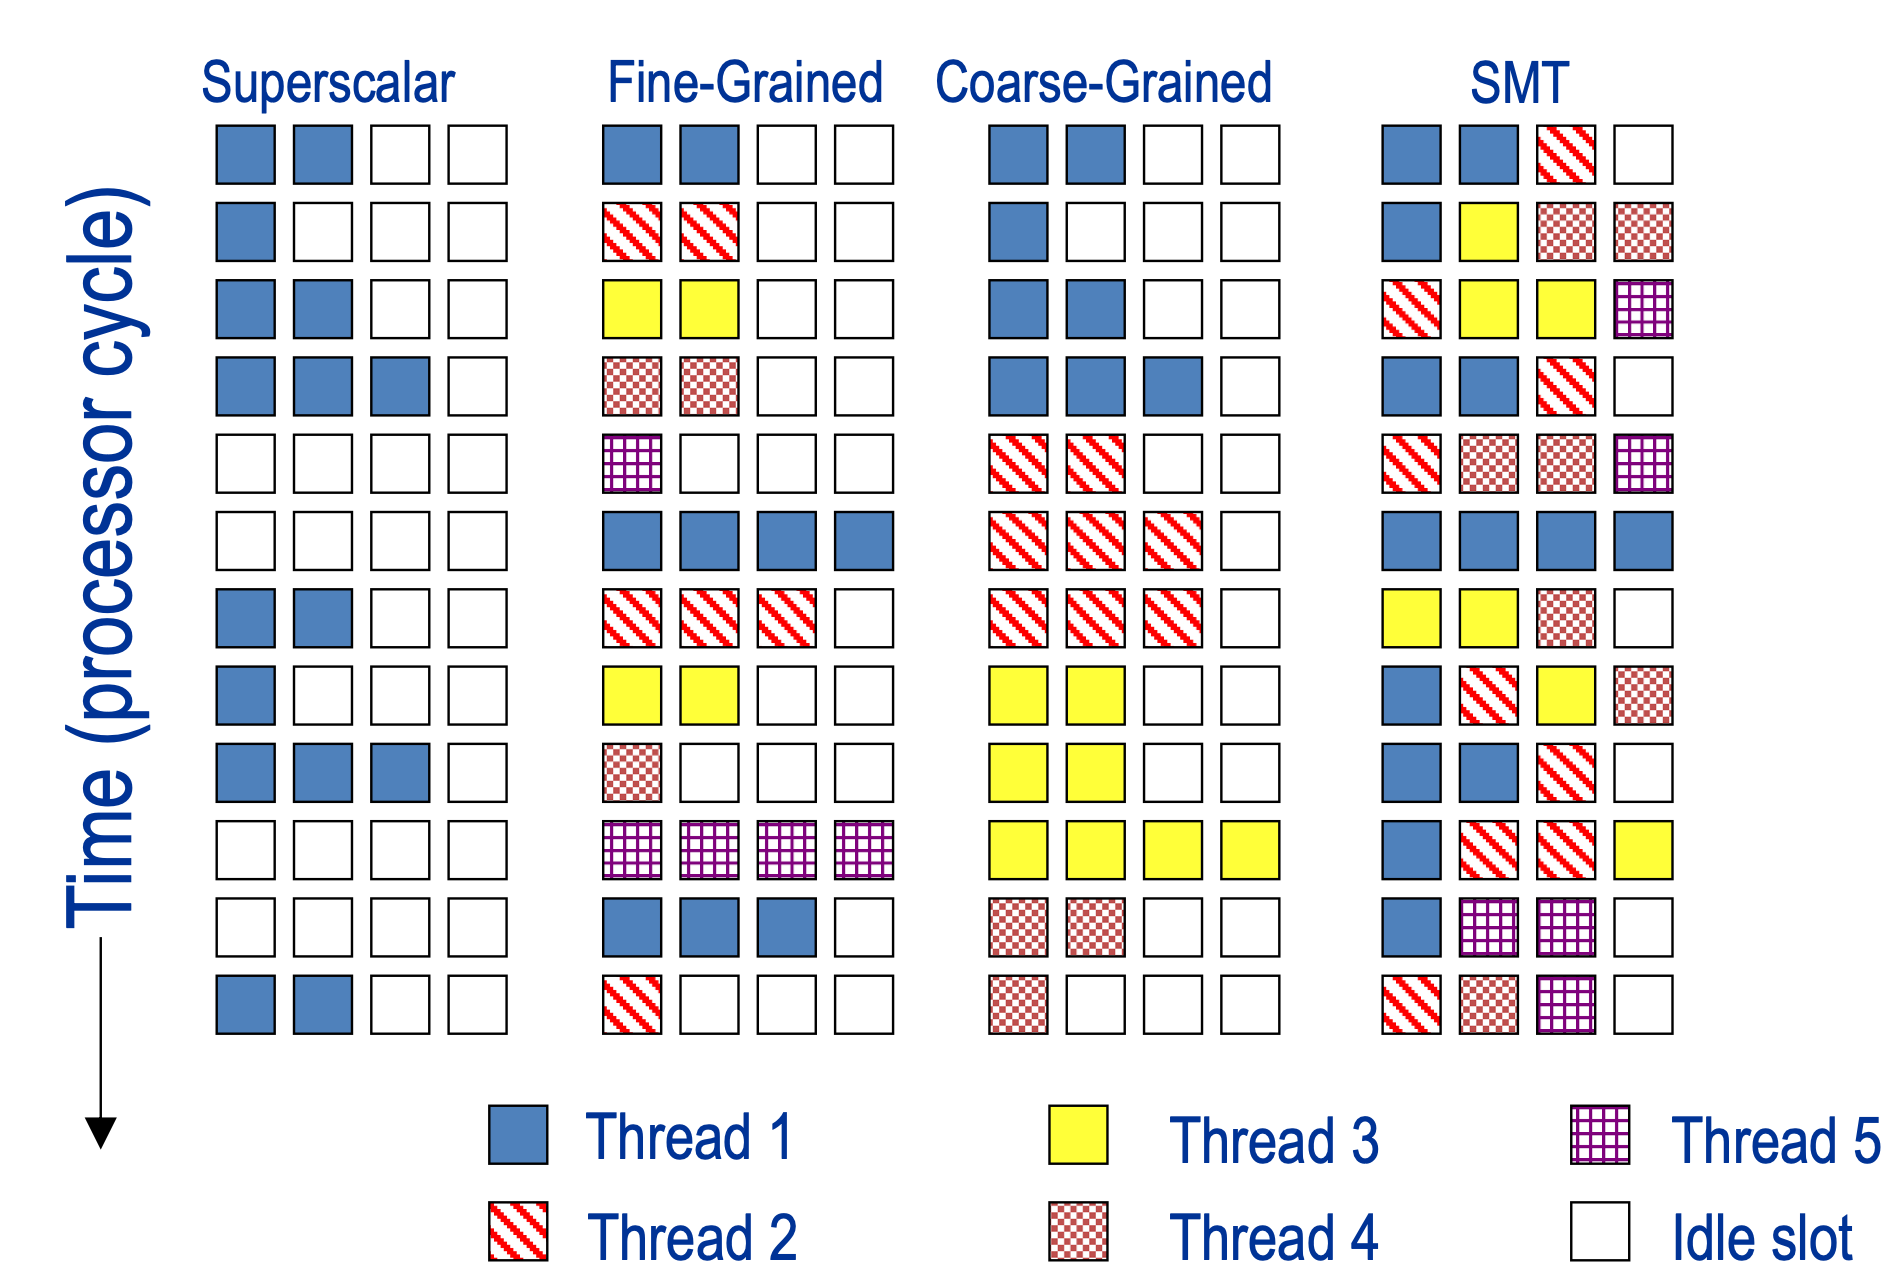
\includegraphics[scale=0.25]{images/multithreaded-categories}
    \caption{Multithreaded categories}
    \label{fig:multithreaded-categories}
\end{figure}

TLP (e.g., superscalar) and ILP (e.g., pipelining) exploit two different forms of parallelism in a program, the
following questions arise:
\begin{itemize}
    \item Could a processor oriented at ILP exploit TLP too?
    \item Functional units are often idle in data path designed for ILP because of either stalls or dependencies in
    the code.
    Could the TLP be used as a source of independent instructions that might keep the processor busy during stalls?
    \item Could TLP be used to employ the functional units that would otherwise lie idle when insufficient ILP exists?
\end{itemize}